%%%%%%%%%%%%%%%%%%%%%%%%%%%%%%%%%%%%%%%%%
% Beamer Presentation
% LaTeX Template
% Version 1.0 (10/11/12)
%
% This template has been downloaded from:
% http://www.LaTeXTemplates.com
%
% License:
% CC BY-NC-SA 3.0 (http://creativecommons.org/licenses/by-nc-sa/3.0/)
%
%%%%%%%%%%%%%%%%%%%%%%%%%%%%%%%%%%%%%%%%%

%----------------------------------------------------------------------------------------
%	PACKAGES AND THEMES
%----------------------------------------------------------------------------------------

\documentclass[aspectratio=169]{beamer}
%\usepackage[ngerman]{babel}
\usepackage{amsmath}
\usepackage{bm}
\usepackage{amssymb}
\usefonttheme[onlymath]{serif}
\mode<presentation> {

% The Beamer class comes with a number of default slide themes
% which change the colors and layouts of slides. Below this is a list
% of all the themes, uncomment each in turn to see what they look like.

\usetheme{default}
%\usetheme{AnnArbor}
%\usetheme{Antibes}
%\usetheme{Bergen}
%\usetheme{Berkeley}
%\usetheme{Berlin}
%\usetheme{Boadilla}
%\usetheme{CambridgeUS}
%\usetheme{Copenhagen}
%\usetheme{Darmstadt}
%\usetheme{Dresden}
%\usetheme{Frankfurt}
%\usetheme{Goettingen}
%\usetheme{Hannover}
%\usetheme{Ilmenau}
%\usetheme{JuanLesPins}
%\usetheme{Luebeck}
\usetheme{Madrid}
%\usetheme{Malmoe}
%\usetheme{Marburg}
%\usetheme{Montpellier}
%\usetheme{PaloAlto}
%\usetheme{Pittsburgh}
%\usetheme{Rochester}
%\usetheme{Singapore}
%\usetheme{Szeged}
%\usetheme{Warsaw}

% As well as themes, the Beamer class has a number of color themes
% for any slide theme. Uncomment each of these in turn to see how it
% changes the colors of your current slide theme.

%\usecolortheme{albatross}
%\usecolortheme{beaver}
%\usecolortheme{beetle}
%\usecolortheme{crane}
%\usecolortheme{dolphin}
%\usecolortheme{dove}
%\usecolortheme{fly}
%\usecolortheme{lily}
%\usecolortheme{orchid}
%\usecolortheme{rose}
%\usecolortheme{seagull}
%\usecolortheme{seahorse}
%\usecolortheme{whale}
%\usecolortheme{wolverine}

%\setbeamertemplate{footline} % To remove the footer line in all slides uncomment this line
%\setbeamertemplate{footline}[page number] % To replace the footer line in all slides with a simple slide count uncomment this line

%\setbeamertemplate{navigation symbols}{} % To remove the navigation symbols from the bottom of all slides uncomment this line
}

\usepackage{graphicx} % Allows including images
\usepackage{booktabs} % Allows the use of \toprule, \midrule and \bottomrule in tables

%----------------------------------------------------------------------------------------
%	TITLE PAGE
%----------------------------------------------------------------------------------------

\title[Smart Services Development]{Implementation of a Home Automation Service} % The short title appears at the bottom of every slide, the full title is only on the title page

\author{Benedikt Görgei, Lukas D'Angelo, Patrick Eder} % Your name
\institute[] % Your institution as it will appear on the bottom of every slide, may be shorthand to save space
{
Technische Universität Graz \\ % Your institution for the title page
\medskip
\texttt{benedikt.goergei@student.tugraz.at, lukas.dangelo@student.tugraz.at, patrick.eder@student.tugraz.at} % Your email address
}
\date{\today} % Date, can be changed to a custom date

\begin{document}

\begin{frame}
\titlepage % Print the title page as the first slide
\end{frame}

\begin{frame}
\frametitle{Overview} % Table of contents slide, comment this block out to remove it
\tableofcontents % Throughout your presentation, if you choose to use \section{} and \subsection{} commands, these will automatically be printed on this slide as an overview of your presentation
\end{frame}

%----------------------------------------------------------------------------------------
%	PRESENTATION SLIDES
%----------------------------------------------------------------------------------------

%------------------------------------------------
\section{Introduction} % Sections can be created in order to organize your presentation into discrete blocks, all sections and subsections are automatically printed in the table of contents as an overview of the talk
%------------------------------------------------
\subsection{Concept}
\begin{frame}
\frametitle{Introduction - Concept}
\begin{itemize}
\item Tiny network enabled device
\item Two relay outputs
\item Two logic inputs
\item One BUS interface for sensors
\item Client - server model
\item MQTT for controlling and sensing
\item TELNET \& serial for configuration 
\end{itemize}
\end{frame}

\begin{frame}
\frametitle{Introduction - Concept}
\begin{figure}
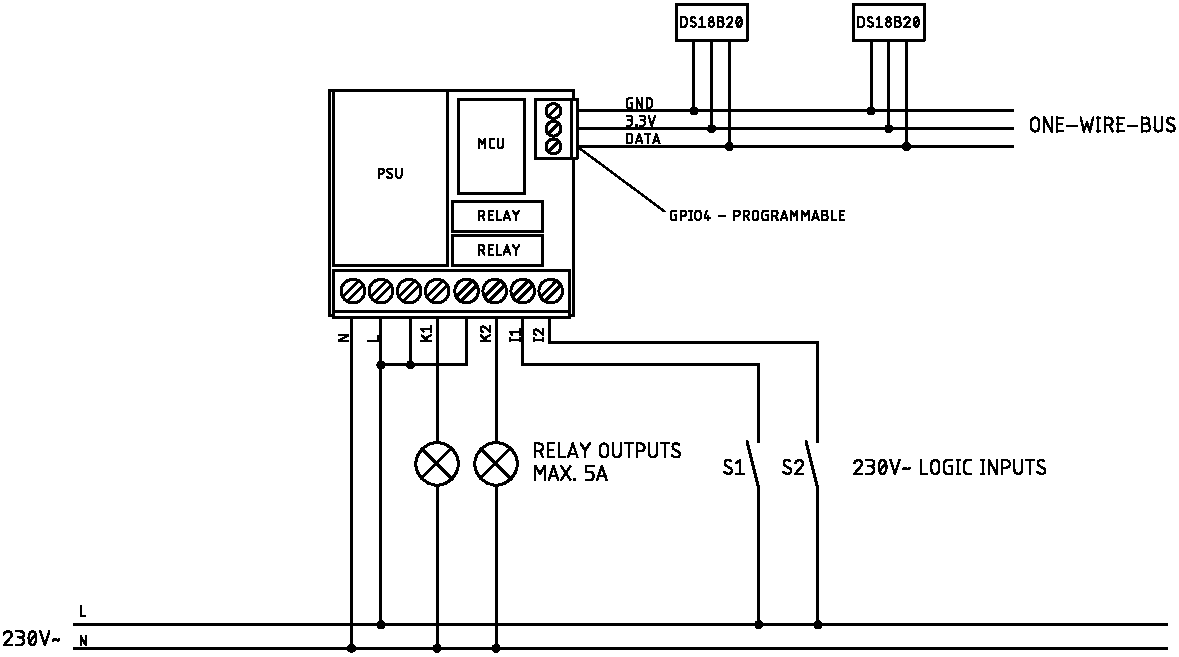
\includegraphics[width=0.6\linewidth]{./figures/concept.pdf}
\end{figure}
\end{frame}

%------------------------------------------------
\section{Hardware}
\subsection{Schematic}
%------------------------------------------------
\begin{frame}
\frametitle{Hardware - Schematic}
\begin{figure}
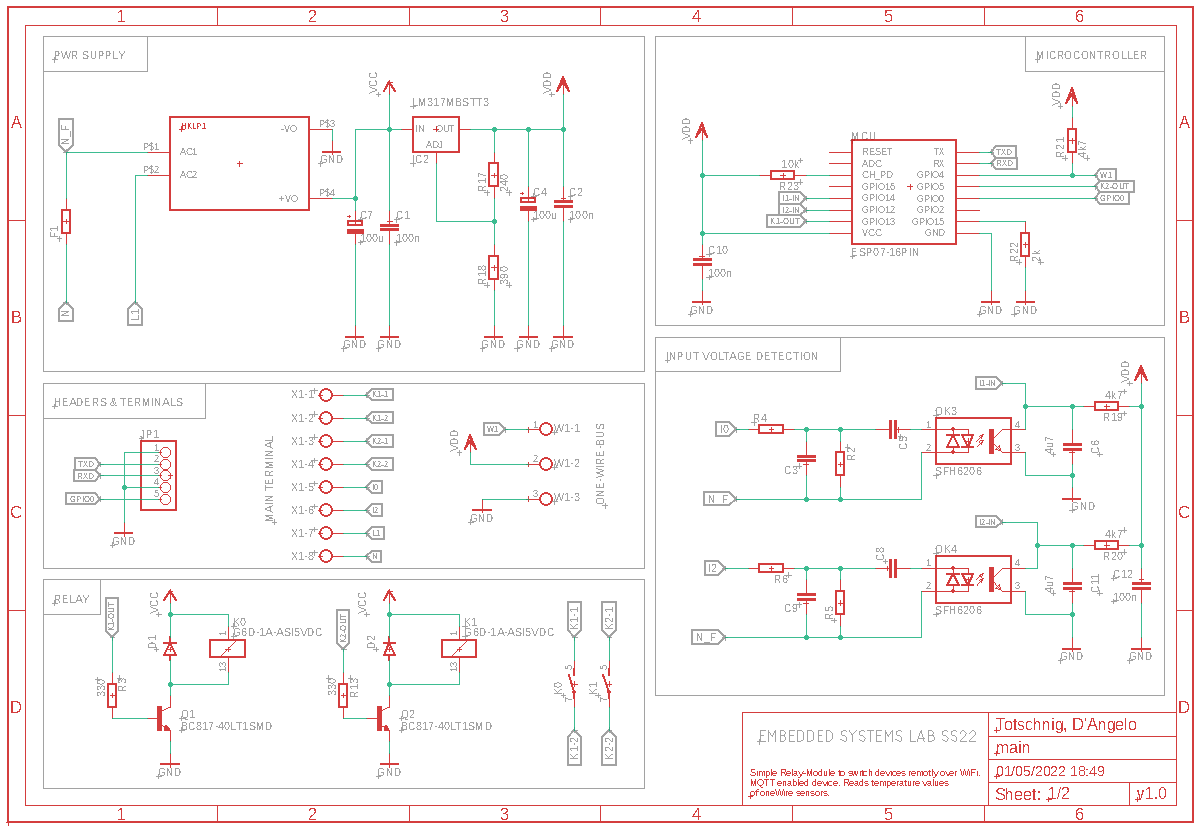
\includegraphics[width=0.65\linewidth]{./figures/schematic.png}
\end{figure}
\end{frame}

%------------------------------------------------
\subsection{PCB Layout}
%------------------------------------------------
\begin{frame}
\frametitle{Hardware - PCB Layout}
\begin{figure}
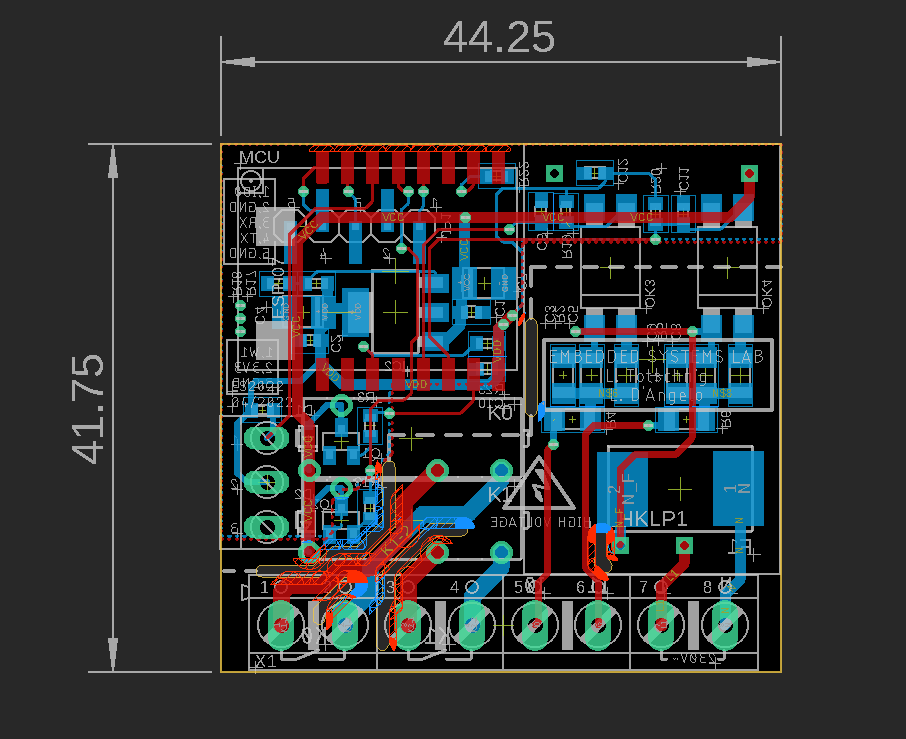
\includegraphics[width=0.5\linewidth]{./figures/layout.png}
\end{figure}
\end{frame}


%------------------------------------------------
\section{Software}
\subsection{Firmware}
%------------------------------------------------
\begin{frame}
\frametitle{Software - Firmware}
\begin{itemize}
\item Framework based on a previous project
\item Simple CLI for configuration \& setup
\item TELNET \& serial for configuration 
\item Client - server model
\item MQTT used for control channel and state channel
\item Firmware upgrade OTA over HTTP
\end{itemize}
\end{frame}

%------------------------------------------------
\section{State of the Project}
\subsection{Current State}
%------------------------------------------------
\begin{frame}
\frametitle{State of the Project - Current State}

\begin{itemize}
 \item[$\boxtimes$] Waiting for feedback                      (10/04/22) 
 \item[$\boxtimes$] Finishing the design of the PCB           (17/04/22) 
 \item[$\boxtimes$] Placing the order on JLCPCB               (17/04/22) 
 \item[$\boxtimes$] Creating a prototype of the firmware      (17/04/22) 
 \item[$\boxtimes$] Preparing the mid-term presentation       (01/05/22) 
 \item[$\boxtimes$] Soldering of the remaining components     (08/05/22) 
 \item[$\boxtimes$] Testing the hardware                      (15/05/22) 
 \item[$\square$] Adding hardware support to firmware       (15/05/22) 
 \item[$\square$] Setting up the test network               (22/05/22) 
 \item[$\square$] Setting up the Raspberry PI               (22/05/22) 
 \item[$\square$] Creation of the demo video                (31/05/22) 
 \item[$\square$] Writing the report                        (31/05/22) 
\end{itemize}
\end{frame}

\begin{frame}
\Huge{\centerline{Thank you!}}
\Huge{\centerline{$\exists$ Questions?}}
\end{frame}

\end{document}